% !TEX root = main.tex

\addtocontents{toc}{\protect\newpage}
\secc[Design]{Design and implementation}

\ssecc{Get familiar with survival models}

\ssecc{Preprocess data}

As it was previously stated the data needs to be preprocessed before start training with it.
This steps are required because small changes can really help in reducing the time needed to
fit the model. Also, by normalizing the data and setting variance to 1 and mean to 0 the network
can converge faster.
~\cite{neural:efficient-backprop}

The whole preprocess task took longer than expected as many tasks required more steps than 
planned. The planned duration was 1 week and the final duration was from March 13\Th and
ended in April 11\Th so its duration was of 4 weeks. However, this wasn't as problematic as 
it could seem since the previous task was completed early.

Also, this task has been done sometimes while doing other tasks because some preprocess 
steps have been added later to improve the network's results.

\sssecc{Image data}

The imaging data in the \Gls{PMHNK} contains 671 folders, each one with the scan of one patient. 
We also have the clinical information of 661 patients, although we do not have a \gls{CT} for
each of the clinical information patients. Through the intersection of each of the two data
sources we have 544 patients with both a \gls{CT} scan and the clinical information.

However, because there was a problem in the way the \gls{CT} scan was computed we only have
the tumour annotations for 509 of the 544 patients, so the data that we can use is reduced
again. \textbf{509} will be the final dataset size that will be used for the next 
steps.

For all the valid patients their directory structure is the same. They contain two folders,
one with all the original scan slices and the other with the slice's tumour mask annotations. 
All the slices are in \verb|.dcm| format.
As an example, the structure for patient \texttt{FHBO0003} can be seen in \autoref{fig:hnk-raw}.

\begin{figure}
  \centering
  \begin{minipage}{0.8\textwidth}
    \begin{Verbatim}[samepage=true]
FHBO003
├── FHBO003           // Original scan
│   ├── IMG0001.dcm
│   ├── IMG0002.dcm
│   ├── ...
│   └── IMG0191.dcm
└── FHBO003-MASS      // Annotated mask
    ├── IMG0001.dcm
    ├── IMG0002.dcm
    ├── ...
    └── IMG0191.dcm
    \end{Verbatim}
  \end{minipage}
    
  \caption{Original data directory structure \label{fig:hnk-raw}}
\end{figure}

Preprocessing the image data requires multiple steps:
\begin{enumerate}
  \item Select valid directories that follow the previously stated conditions
  \item Join all the \verb|.dcm| files into a 3D \verb|numpy| array
  \item Apply gaussian filter to mask image. This is done because the mask is manually annotated
        and usually each layer does not fit perfectly with the previous one. This way a smooth
        transition between layers is ensured.
  \item Get 3D bounding box containing the tumour.
  \item Slice original image and mask with the bounding box to extract the parts only containing
        the tumour. A single bounding box is obtained.
  \item Remove extreme values, if the value of the image is smaller than -1000 or bigger than
        400 this means that this are pixels usually outside of the scanner. This happens because
        the scanner has a circular field of view but a squared image is generated instead, so 
        all the pixels outside the circle are \emph{error pixels}.
  \item Apply mask to extracted image. Since the mask only contains 1s and 0s it's as easy 
        as \verb|image *= mask|.
  \item Resize the sliced image to a size of \( 64 \times 64 \times 64 \)
  \item Normalize image by setting mean = 0 and variance = 1. It's done in the following way:
  \begin{itemize}
    \item \verb|image -= mean(image)|
    \item \verb|image /= std(image)|
  \end{itemize}
  \item Rotate the image 3 times to get 4 different versions of the scan that can be used for 
        training as data augmentation.
\end{enumerate}

\begin{figure}
  \resizebox{\textwidth}{.7\textwidth}{
    \def\customimage{10em}
\begin{tikzpicture}[node distance = 2]
    \node (P-0) at (0, 0) {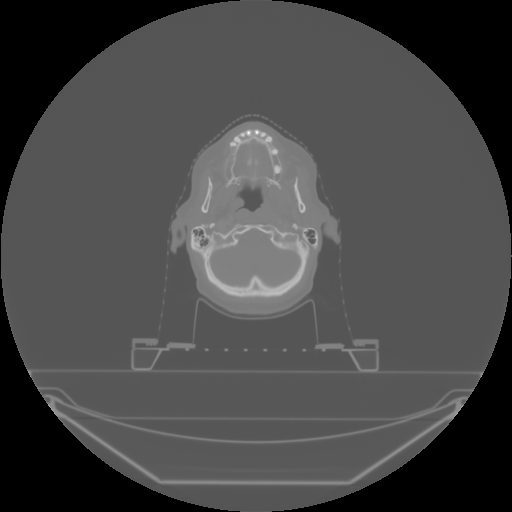
\includegraphics[width=\customimage]{images/preprocess/process_0}};
    \node [below = of P-0] (P-1) {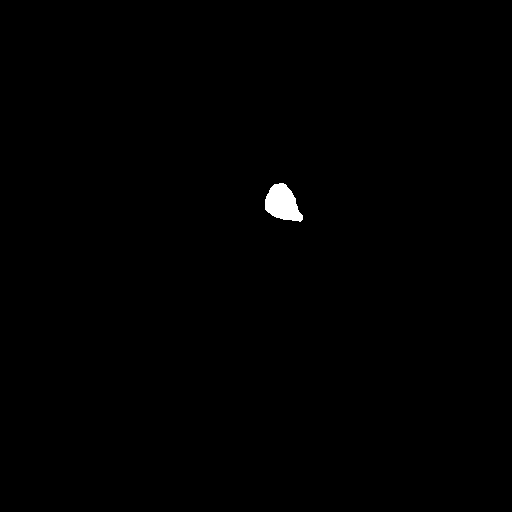
\includegraphics[width=\customimage]{images/preprocess/process_1}};

    \node [below = .2 of P-0] (text-0) {Scan};
    \node [below = .2 of P-1] (text-1) {Mask};
    
    \node [right = of P-1] (P-2-0) {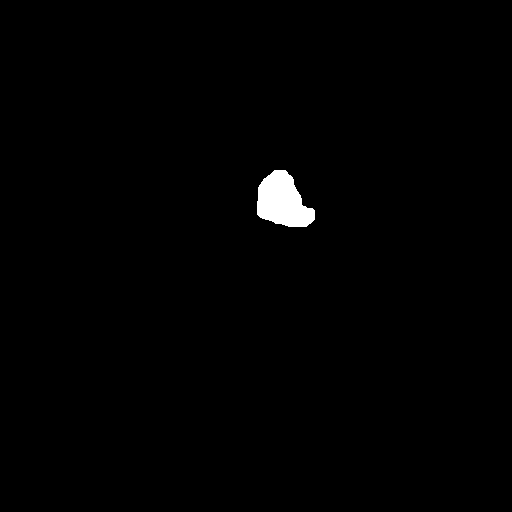
\includegraphics[width=\customimage]{images/preprocess/process_2_0}};
    \node [right = of P-2-0] (P-2-1) {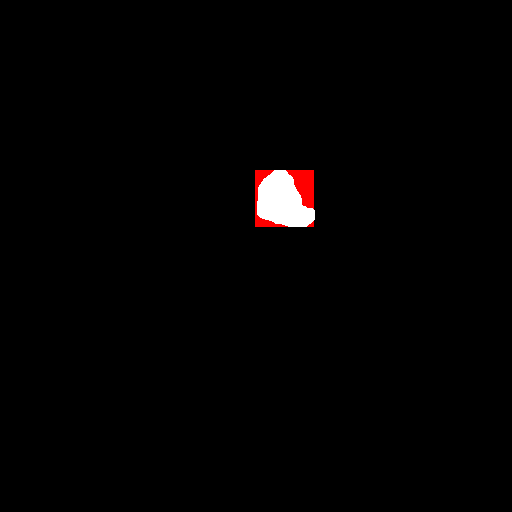
\includegraphics[width=\customimage]{images/preprocess/process_2_1}};
    \node [right = of P-2-1] (P-5) {
\includegraphics[width=\customimage]{images/preprocess/process_5}};
    
    \node [above = of P-2-1] (P-3) {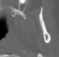
\includegraphics[width=\customimage]{images/preprocess/process_3}};
    \node [right = of P-3] (P-4) {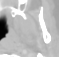
\includegraphics[width=\customimage]{images/preprocess/process_4}};

    \node [right = .5 of P-5, circle, draw] (prod) { \Large \( \times \) };
    
    \node [below = of P-5] (P-6) {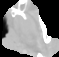
\includegraphics[width=\customimage]{images/preprocess/process_6}};
    \node [left = of P-6] (P-7) {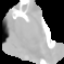
\includegraphics[width=\customimage]{images/preprocess/process_7}};
    \node [left = of P-7] (P-8) {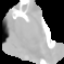
\includegraphics[width=\customimage]{images/preprocess/process_8}};

    \node [below = .2 of P-6] { \( 59 \times 57 \) px};
    \node [below = .2 of P-7] { \( 64 \times 64 \) px};
    \node [below = .2 of P-8] { \( 64 \times 64 \) px};

    \draw [-latex] (P-0) -- (P-3);
    \draw [-latex] (P-3) -- (P-4) node[midway, below, align=center] {Remove \\ extreme \\ values};
    \draw [-latex] (P-4) -| (prod);

    \draw [-latex] (P-1) -- (P-2-0) node[midway, below, align=center] {Gaussian \\ filter};
    \draw [-latex] (P-2-0) -- (P-2-1) node[midway, below, align=center] {Bounding \\ box};
    \draw [-latex] (P-2-1) -- (P-3) node[midway, right, align=center] {Slice};
    \draw [-latex] (P-2-1) -- (P-5) node[midway, below, align=center] {Slice};
    \draw [-latex] (P-5) -- (prod);

    \draw [-latex] (prod) |- (P-6) node[near end, below, align=center] {Apply \\ mask};
    \draw [-latex] (P-6) -- (P-7) node[midway, below, align=center] {
        Resize \\ \( 64 \times 64 \times 64 \)
    };

    \draw [-latex] (P-7) -- (P-8) node[midway, below, align=center] {Normalize};

\end{tikzpicture}
  }

  \caption[Image pre-process pipeline]{
    Image pre-process pipeline \label{fig:preprocess}
    
    In this example the process is shown for a 2D image, all the pictures are being resized to 
    have the same size so the steps can be appreciated. The normalization step is not shown as is,
    since setting a mean of 0 and variance of 1 produces an invalid \acrshort{PNG} image, but still valid
    for \gls{ML} purposes.
  }
\end{figure}

\sssecc{Scalar data}

There are two types of scalar data:
\begin{itemize}
  \item Clinical information
  \item Radiomic features extracted from the image, regarding tumour shape, intensity, volume...
\end{itemize}

The clinical information should be anonymized as much as possible and especially if it's going
to be outside \gls{UHN}, the network of hospitals where this project is being developed.
Since this is the case, as the training will be done at \gls{CC} cluster, the unnecessary fields
are removed and only those being used are kept. Moreover, removing the unused fields
is helpful when using the data.

Originally, the clinical information provides 36 different fields. From these fields only the 
following ones are kept:
\begin{itemize}
  \item ID
  \item Age
  \item Sex
  \item Survival event. This one needs to be negated since, in the provided event, \verb|event = 1|
        means survival, but in our survival model this means death. 
  \item Survival time
\end{itemize}

The radiomic features can be extracted directly with the \emph{PyRadiomics}
\cite{medical:py-radiomics} package, but in this case they have been already extracted and stored
in a single file so we can reuse them. These features should be normalized before start training,
because otherwise the network may never converge, which indeed it happened. 

For this normalization to be valid, the mean and the standard deviation are obtained only from 
the train samples. These are different for each feature because not all the features need to 
be normalized in the same way. Afterwards, the normalization is applied to both the train 
and test samples. The mean for the test samples is never obtained, because, otherwise, the
model could have \gls{leakage}. An example of features normalization can be seen in
\autoref{fig:feature-normalization}

\begin{figure}
  \centering

  \begin{subfigure}[t]{.49\textwidth}
    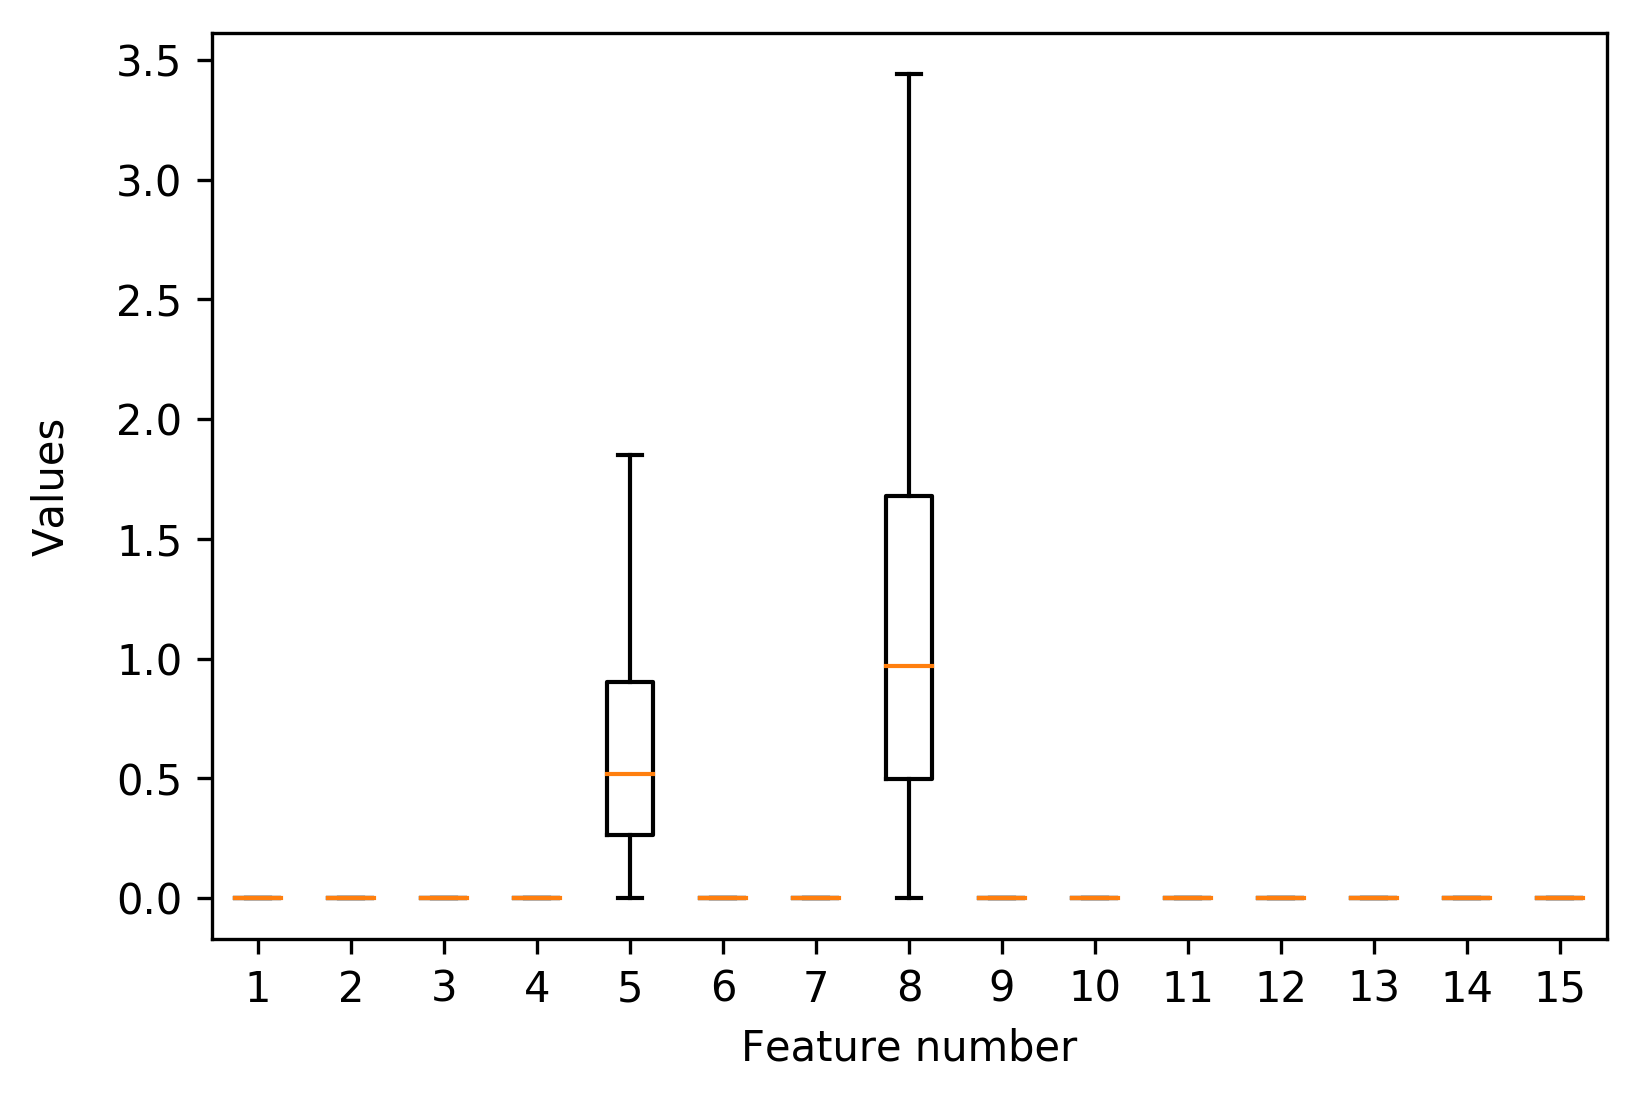
\includegraphics[width=\textwidth]{images/features_original}

    \caption{Features' box plot before normalization \label{fig:feature-normalization-before}}
  \end{subfigure}
  \hfill
  \begin{subfigure}[t]{.49\textwidth}
    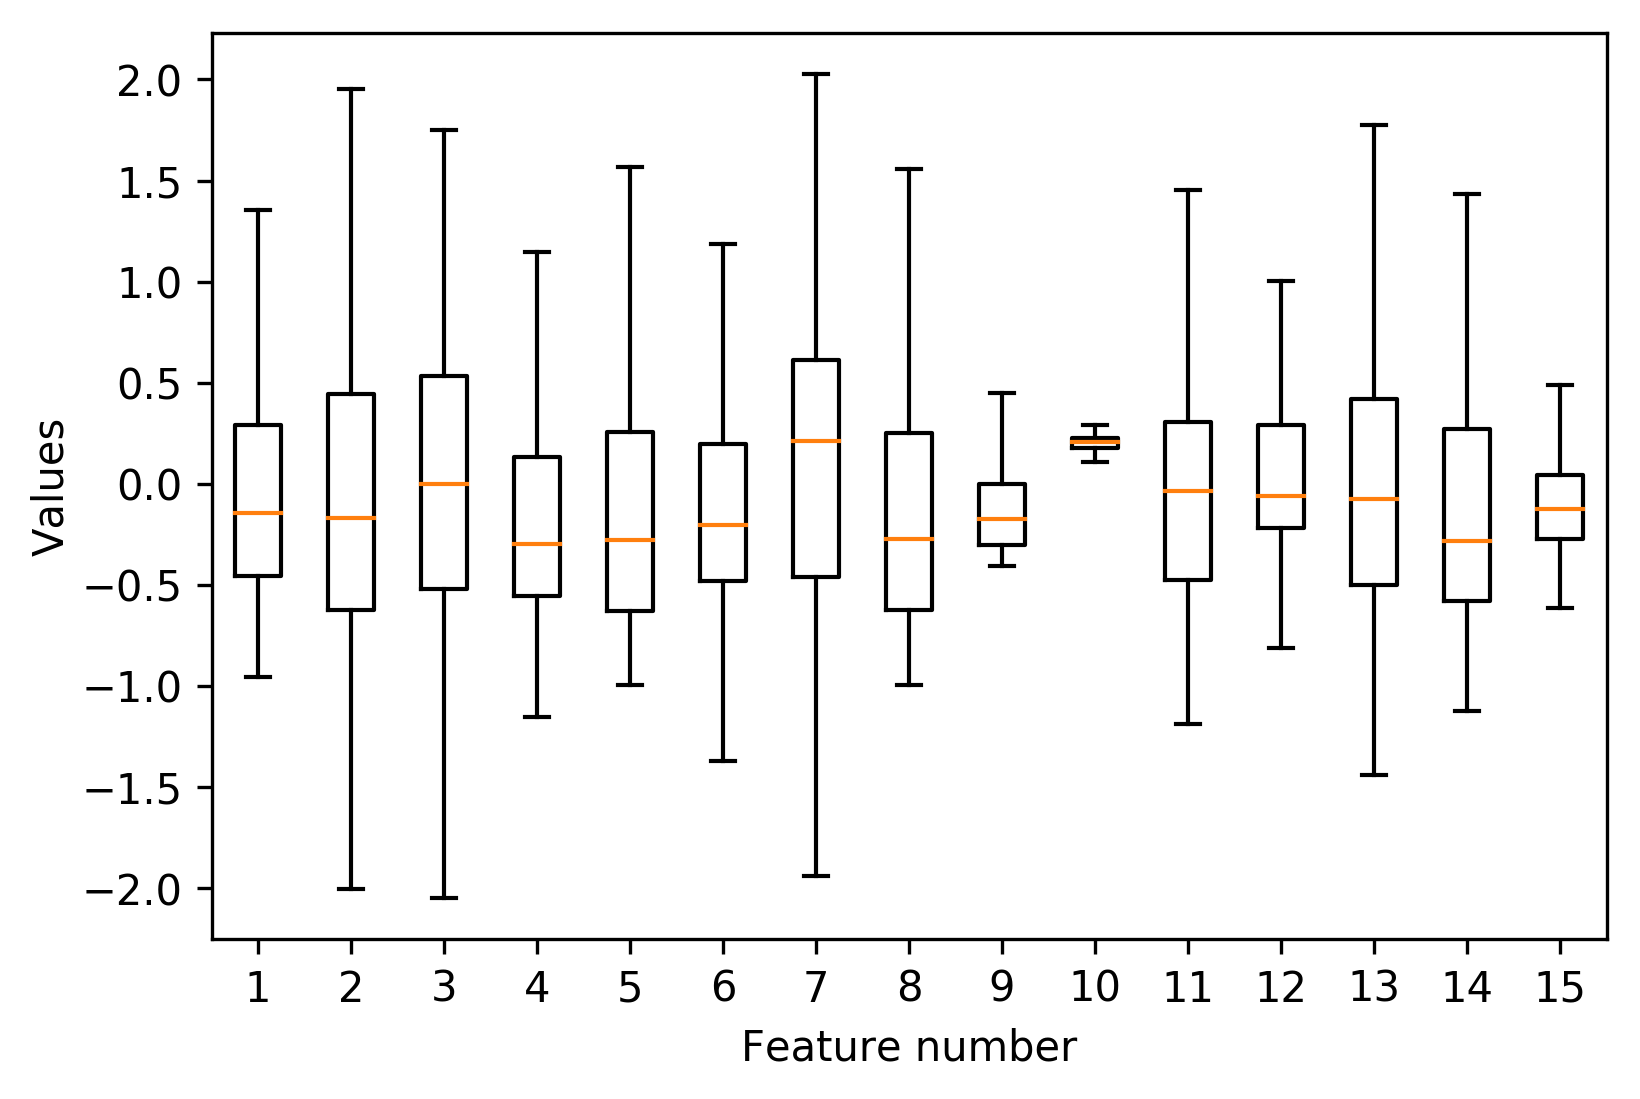
\includegraphics[width=\textwidth]{images/features_normalized}

    \caption{Features' box plot after normalization}
  \end{subfigure}

  \caption[Features normalization example]{
    Features normalization example \label{fig:feature-normalization}
    
    In this example only the first 15 of 725 features are shown for readability. 
    \autoref{fig:feature-normalization-before} shows the features before normalizing them. 
    There, many of the features are too small compared with the ones shown so only a small 
    line is drawn.
  }
  
\end{figure}


\sssecc{Pair generation}

As the siamese network is prepared to train in pairs these have to be generated before. As
it has been explained in \autoref{sec:survival} and shown in \autoref{fig:graph-ci},
for two subjects \( A \) and \( B \) a pair can only be generated if:
\begin{itemize}[noitemsep, topsep=0pt]
  \item Both of them are uncensored (\( E_A = E_B = 1\))
  \item The uncensored time of one is smaller than the censored survival time of the other
  (\( T_A < T_B | E_A = 1; E_B = 0 \))
\end{itemize}

These conditions are to be kept in mind when generating the pairs. Moreover, before starting
the train and test sets must be decided first. Once they have been generated then the pairs
can be generated too. To avoid \gls{leakage} three types of pairs will be defined and will be
used in different contexts:
\begin{description}
  \item[\Gls{train-pair}] \glsdesc*{train-pair}
  \item[\Gls{test-pair}] \glsdesc*{test-pair}
  \item[\Gls{mixed-pair}] \glsdesc*{mixed-pair}
\end{description}

\begin{figure}
  \centering

  \def\customimage{5em}
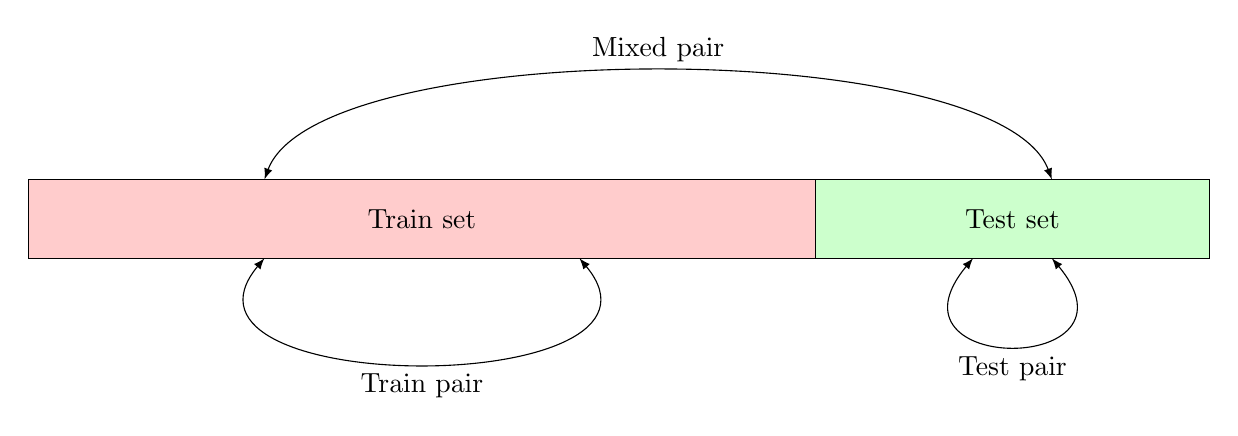
\begin{tikzpicture}
    
    \draw [fill = red!20] (0, 0) rectangle (10, 1);
    \draw [fill = green!20] (10, 0) rectangle (15, 1);

    \node at (5, .5) {Train set};
    \node at (12.5, .5) {Test set};

    \draw [bend right=130, latex-latex, looseness=1.5] (3, 0) to node [midway, below] {Train pair} (7, 0);
    \draw [bend right=130, latex-latex, looseness=5] (12, 0) to node [midway, below] {Test pair} (13, 0);
    \draw [bend left=70, latex-latex, looseness=.5] (3, 1) to node [midway, above] {Mixed pair} (13, 1);
\end{tikzpicture}

  \caption{Types of pairs generated from the test and train sets}
\end{figure}


\ssecc{Create basic siamese model}
\label{sec:basic-siamese}

The first step is to create an environment where different sisters networks can be tested
for improvements. To do so, the loss and cost functions are defined assuming an output
\( \bm{O} \) for the input \( \bm{X} \) of the sister network. This will be called the
basic model.

The distance comparison used for the following siamese networks is defined comparing the 
absolute distance of the sister's output features and then applying the logistic function 
into it to get an output value \( d \in [0, 1] \). This way if it's 1 it means \( T_B > T_A \).
\begin{align*}
  \bm{O}_A &= \operatorname{sister}(\bm{X}_A) \\
  \bm{O}_B &= \operatorname{sister}(\bm{X}_B) \\
  \sigma(x) &= \frac{1}{1 + \exp(-x)} \\
  d &= \sigma(||\bm{O}_B||_2 - ||\bm{O}_A||_2) 
\end{align*}

The loss function used for the model is the log-loss:
\[
  \mathcal{L}(\bm{y}, \hat{\bm{y}}) = -\frac{1}{N} \sum_{i = 1}^{N}
  (1 - y_i)\log(1 - \hat{y}_i) + y_i\log(\hat{y}_i)
\]

The model uses L2 regularization, so the model's cost function, 
adding the regularization loss, is:
\[
  C(\bm{y}, \hat{\bm{y}}) = \mathcal{L}(\bm{y}, \hat{\bm{y}}) + 
  ||\bm{w}||_2
\]

This step was not included in the planning but it was later found that it was necessary to be 
able to test multiple models. The whole process took one week to complete.

\ssecc{Build volume only model}

To be able to have a baseline and compare the results, not only with the state-of-the art ones
but with future designs too, a model using only the most prognostic feature, the volume, is 
built.

This design is a siamese network too and implements the sister network part. The model to fit
is inspired by the idea "A bigger tumour volume means less chances of 
survival" and it is the following one:
\[
  \operatorname{sister}(x) = w\cdot x + b
\]
Where \( x \) in this case is only the volume. This model is built only to set a 
baseline for improvement.

This step was not included in the planning but having a baseline was required to see the 
improvement of the new models compared against this one. This step took half a week to complete,
including the time to test and obtain the results.

\sssecc{Results}

The results with this model have been obtained using both 4-CV and \gls{LOOCV}.
As seen in \autoref{tab:volume-4CV}, when using 4-CV. The final \gls{CI} with mixed pairs
is 0.638. Moreover, it's very similar for the the sets of pairs.

\begin{table}
  \centering
  \begin{tabular}{|c||c|c|c||c|c|c|}
    \cline{2-7}
    \multicolumn{1}{c|}{} & \multicolumn{3}{|c||}{\textbf{Pairs}} & 
    \multicolumn{3}{c|}{\textbf{Concordance Index}} \\
    \hline
    \textbf{Fold} & \textbf{Mixed} & \textbf{Train} & \textbf{Test} 
    & \textbf{Mixed} & \textbf{Train} & \textbf{Test} \\
    \hhline{=======}
    0 & 55512 & 82518 & 9254 & 0.65 & 0.625 & 0.673 \\
    1 & 55176 & 82958 & 9150 & 0.633 & 0.643 & 0.619 \\
    2 & 54864 & 83416 & 9004 & 0.655 & 0.621 & 0.687 \\
    3 & 55576 & 82396 & 9312 & 0.615 & 0.661 & 0.568 \\
    \hhline{=======}
    \textbf{Total} & 221128 & 331288 & 36720 & 0.638 & 0.638 & 0.636 \\
    \hline
  \end{tabular}

  \caption{Results for volume only model using 4-CV \label{tab:volume-4CV}}
\end{table}

The results obtained with \gls{LOOCV} are shown in \autoref{fig:results-volume-LOOCV}. 
To train this model one element has been removed from the dataset and the model has 
been trained with the rest of the elements (all minus one). It shows the \gls{CI} of each
element when comparing it with the training set, so only the mixed pairs \gls{CI} are shown.

In this case the distribution of the censored data is important because many censored elements
can create very few pairs (< 100) so they may give a wrong sense of security when looking at
the \gls{LOOCV}. As it can be seen the 
distribution for the uncensored data is quite similar from the rest of the dataset. 
The final \gls{CI} is 0.638 and the mean \gls{CI} is 0.647. A distribution of the number of
pairs for each element compared against its \gls{CI} can be seen in \autoref{fig:scatter-volume-CI}.

This results are very similar from the ones previously obtained of 0.628 as explained in the
state-of-the art.

\begin{figure}
  \centering
  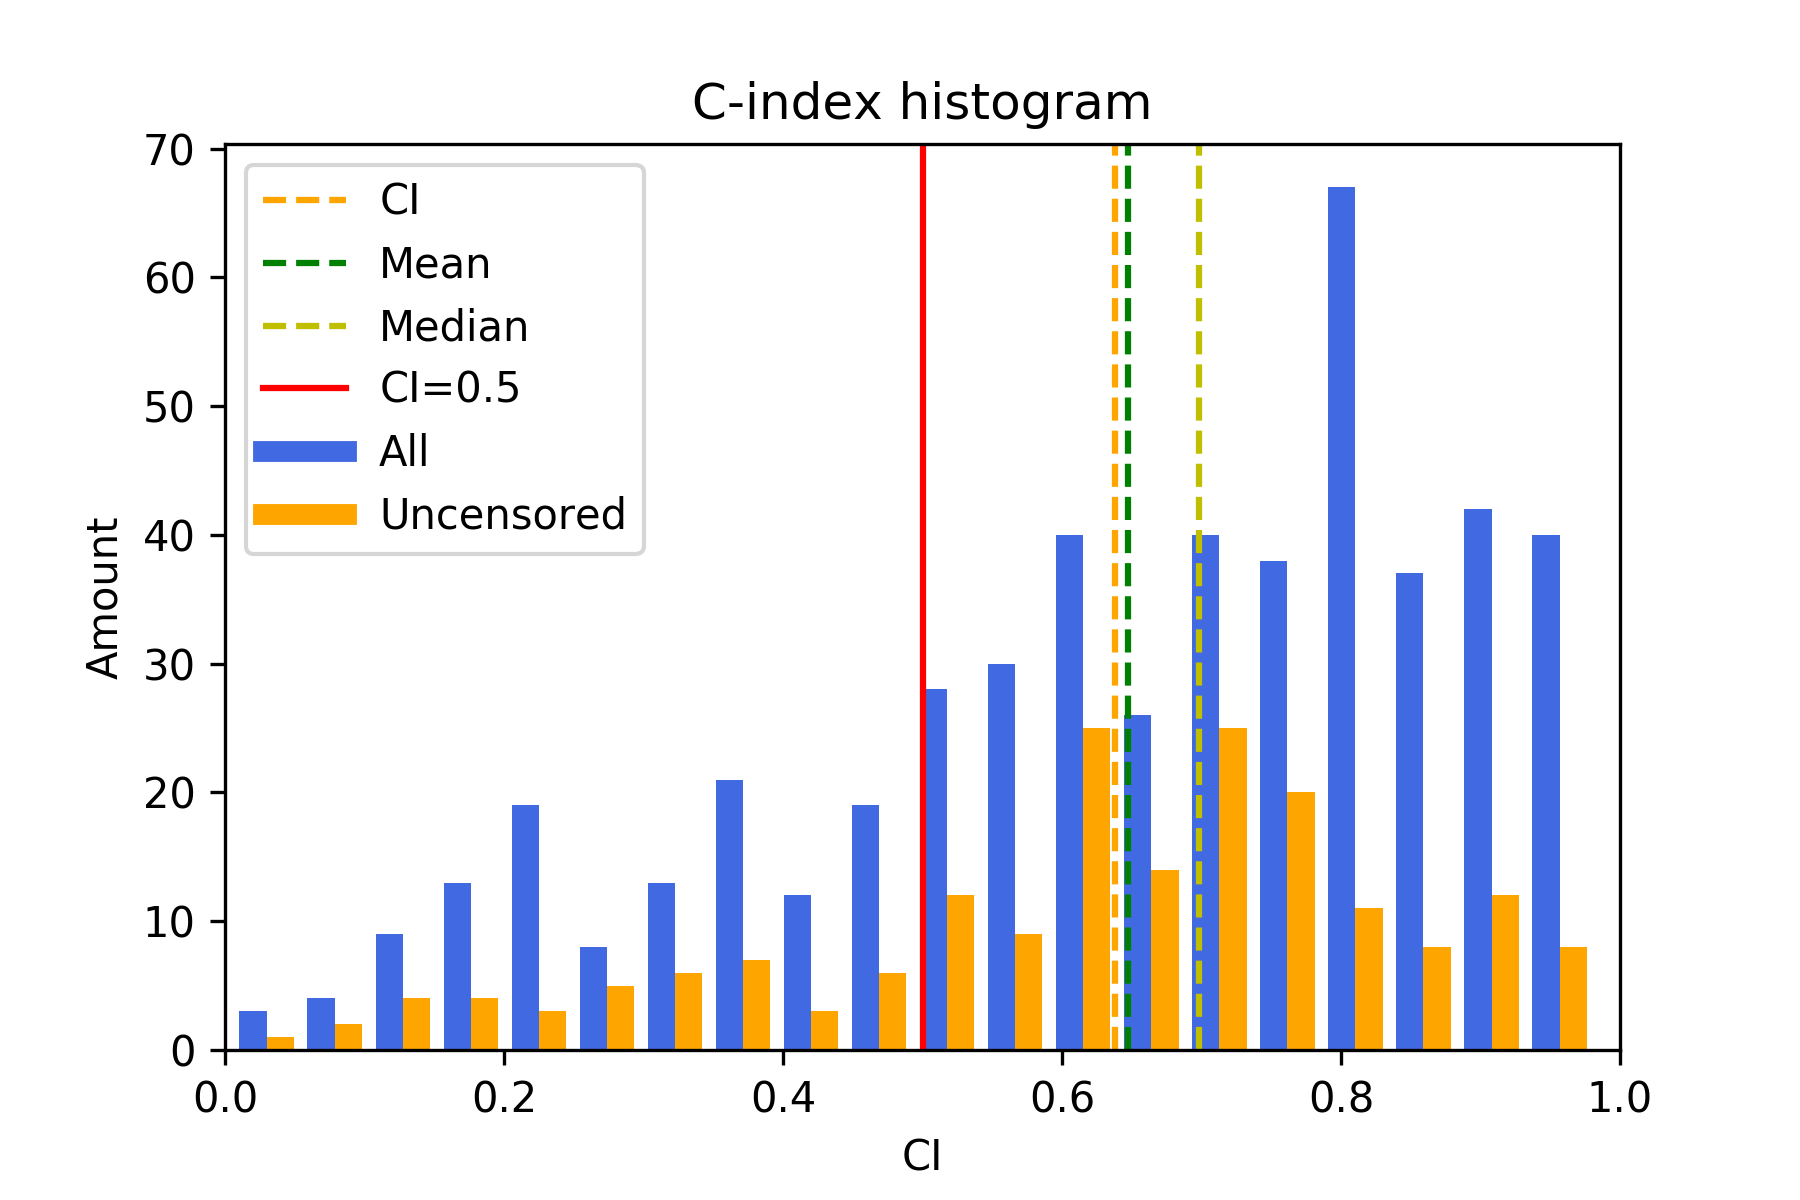
\includegraphics[width=.8\textwidth]{images/results/c-index_volume}
  \caption[LOOCV volume only model results]{
    Volume only model results using \acrshort{LOOCV} \label{fig:results-volume-LOOCV}
    
    Histogram showing the distribution of all the \acrshort{LOOCV} elements' \acrshort{CI}
    when using mixed pairs to obtain the \acrshort{CI}. 
    In blue the distribution of all the \acrshort{LOOCV} elements. In orange only the uncensored
    elements, which have more pairs to compare with.
  }
\end{figure}
\begin{figure}
  \centering
  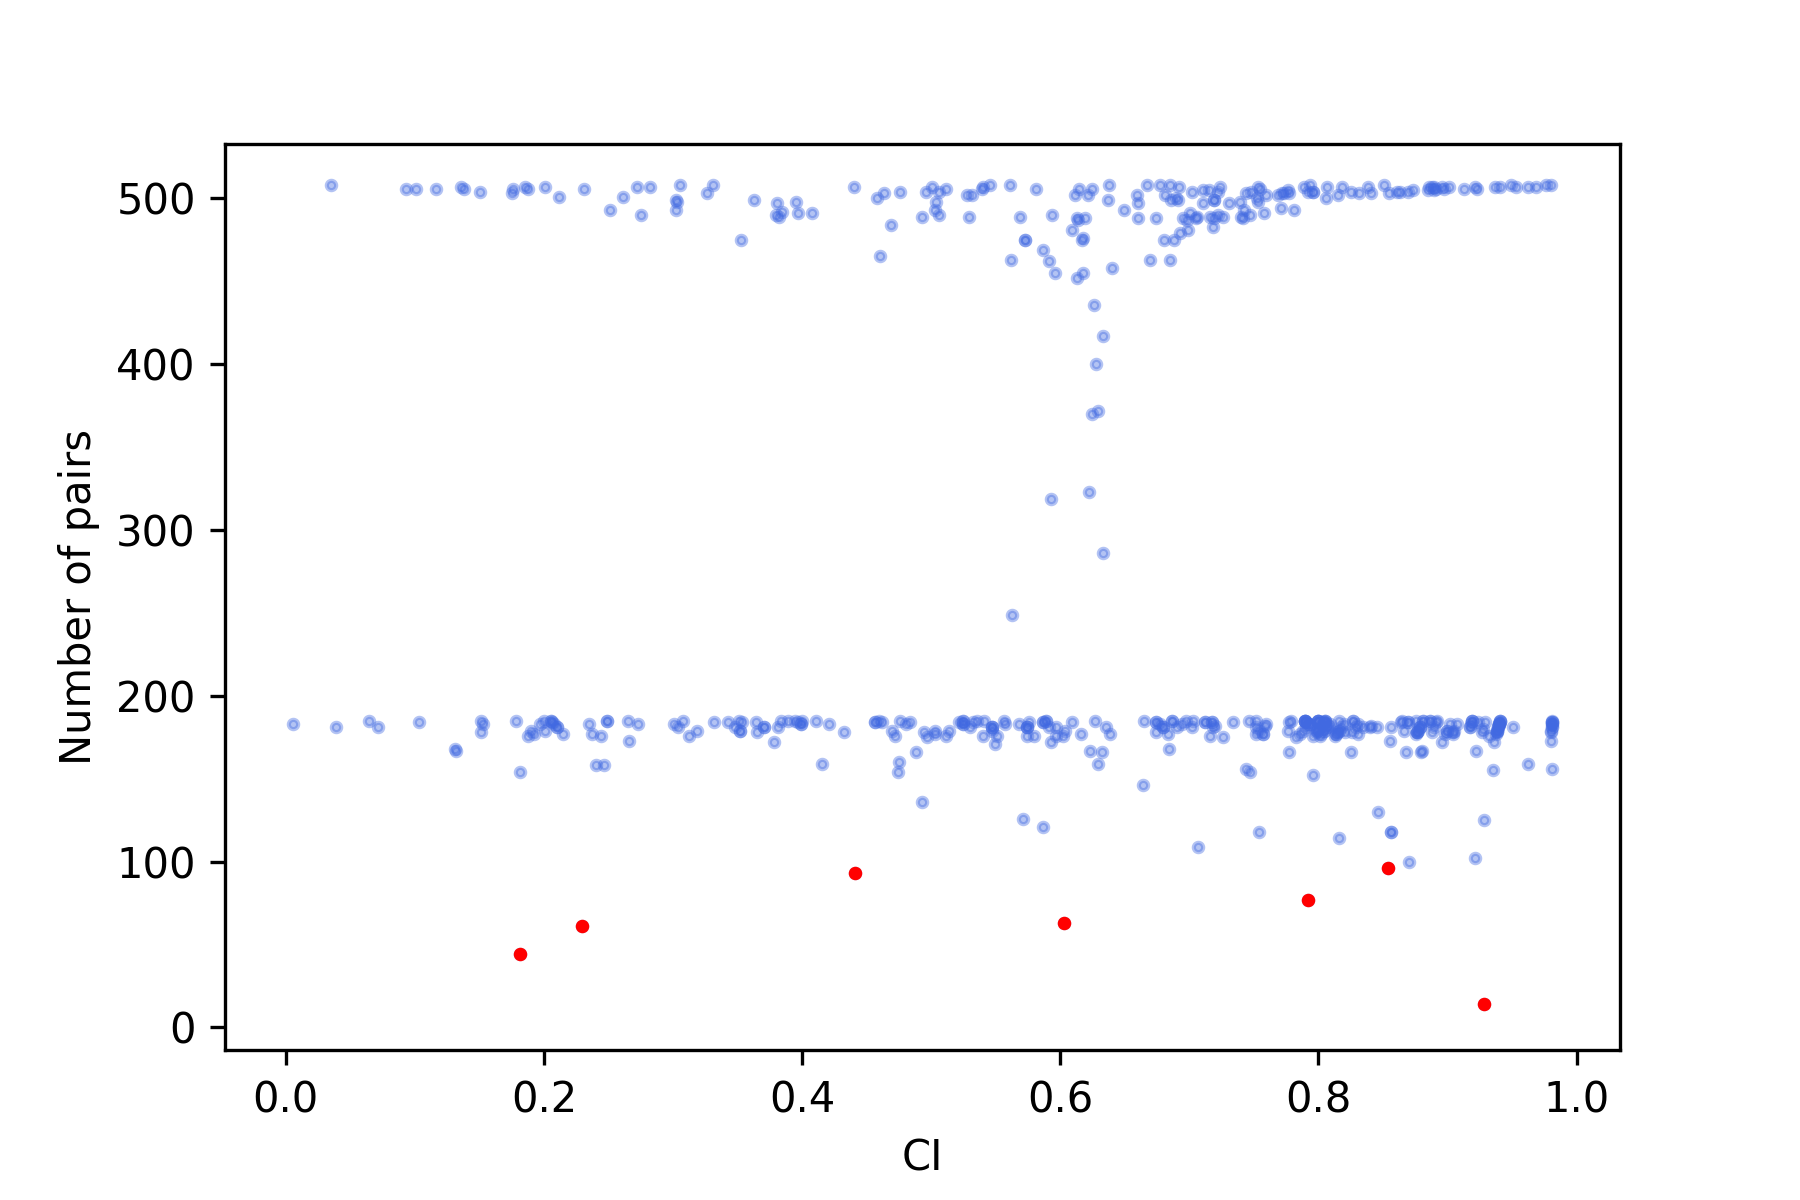
\includegraphics[width=.8\textwidth]{images/results/scatter_volume}
  \caption[CI against pairs scatter plot]{
    Scatter plot of \acrshort{CI} against number of pairs for volume only model
    \label{fig:scatter-volume-CI}
  }.
\end{figure}

\ssecc{Build shallow siamese network}
\label{sec:shallow-siamese}

The initial shallow siamese network design had a very simple design for the sister network. 
In fact, it was so simple that a proper \gls{CNN} could not be build, the original design 
can be found in \autoref{fig:shallow-sister}.

The main problem was that there were only two convolutional layers so that when trying to reduce
the image dimension the output image still was too big for a Fully Connected layer. With this
problem in mind a new design was made and it's shown in \autoref{fig:shallow-implement}.

This new design has more layers to reduce the dimensions of the image and is able to 
incorporate the scalar data. As it was previously said this design it's still part of the
siamese network model.

Some initial results have been obtained with this model although these are still not valid as
this task has been scheduled for completion in a later step of the project. The cause of the 
rescheduling is due to the long training times. Once a more basic model is working and
with some results, this task will be finished.

This has been developed for two weeks for now and it will take at least one more to complete.
Since this step has taken less time than planned it has made some room to add other required
steps that were not planned initially.

\begin{figure}
  \centering
  
\begin{tikzpicture}[every node/.style={scale=.8}]

  \tikzstyle{module}=[rounded corners, draw, align=center]
  \tikzstyle{FC}=[module, fill=green!30]
  \tikzstyle{conv}=[module, fill=orange!30]
  \tikzstyle{io}=[module, fill=purple!30]
  
  
  \node [io] (image) {Image};
  \node [conv, below = of image] (CNN-1) at (0, 0) {
    Convolution 1 \\ 
    \( 30 @ 3 \times 3 \times 3 \) \\
    Stride = 2
  };
  \node [conv, below = of CNN-1] (CNN-2) {
    Convolution 2 \\
    \( 30 @ 3 \times 3 \times 3 \) \\
    Stride = 2
  };
  \node [conv, below = of CNN-2] (CNN-3) {
    Convolution 3 \\
    \( 40 @ 3 \times 3 \times 3 \)
  };
  \node [conv, below = of CNN-3] (CNN-4) {
    Convolution 4 \\
    \( 40 @ 3 \times 3 \times 3 \)
  };
  \node [conv, below = of CNN-4] (CNN-5) {
    Convolution 5 \\
    \( 50 @ 3 \times 3 \times 3 \)
  };

  \node [right = 5 of image] (aux) {};
  \node [io, right = of aux] (scalar) {Scalar};

  \node [FC, below = of aux] (con) {Concatenate + \\ flatten};
  \node [left = of con] (aux-2) {};
  \node [FC, below = of con] (FC-1) {FC \\ 8000 units};
  \node [FC, below = of FC-1] (FC-2) {FC \\ 1000 units};
  \node [FC, below = of FC-2] (FC-3) {FC \\ 10 units};

  \node [io, below = of FC-3] (out) {Sister out};
  
  \draw [-latex] (image) -- (CNN-1) node[midway, right] {\( 64 \times 64 \times 64 \times 1 \)};
  \draw [-latex] (CNN-1) -- (CNN-2) node[midway, right] {\( 31 \times 31 \times 31 \times 30 \)};
  \draw [-latex] (CNN-2) -- (CNN-3) node[midway, right] {\( 15 \times 15 \times 15 \times 40 \)};
  \draw [-latex] (CNN-3) -- (CNN-4) node[midway, right] {\( 13 \times 13 \times 13 \times 40 \)};
  \draw [-latex] (CNN-4) -- (CNN-5) node[midway, right] {\( 11 \times 11 \times 11 \times 40 \)};

  \draw (CNN-5) -| (aux-2.center)  node[pos=.3, below] {\( 9 \times 9 \times 9 \times 50 \)};
  \draw [-latex] (aux-2.center) |- (con);
  \draw [-latex] (scalar) |- (con) node[pos=.15, left] {\( 725 \)};
  
  \draw [-latex] (con) -- (FC-1) node[midway, right] {\( 37.175 \)};
  \draw [-latex] (FC-1) -- (FC-2) node[midway, right] {\( 8000 \)};
  \draw [-latex] (FC-2) -- (FC-3) node[midway, right] {\( 1000 \)};
  \draw [-latex] (FC-3) -- (out) node[midway, right] {\( 10 \)};
\end{tikzpicture}



  \caption{Shallow siamese sister's network illustration \label{fig:shallow-implement}}
\end{figure}


\ssecc{Build scalar only siamese network}
\label{sec:scalar-only}

To speed up the testing process, a siamese network that only used scalar features 
was built. With this approach, the training time was reduced from around 5 hours 
to 1 minute to train the model. 

To improve the performance Dropout \cite{neural:dropout} was used, by using dropout some 
of the model activations are zeroed and then scaled according to the dropout probability. 
This way, the networks' neurons do not have all the information and thus they must generalize. 
Dropout is used as a way of regularization. 

Moreover, since this model inherits from the basic model, defined in \autoref{sec:basic-siamese}, 
regularization is applied too by adding the l2 norm of the weights. The loss and
cost functions are the same too.

This step took one week to complete although some fixes have been applied later during the
development of other models.

\begin{figure}
  \centering
  
\begin{tikzpicture}[every node/.style={scale=.8}]

  \tikzstyle{module}=[rounded corners, draw, align=center]
  \tikzstyle{FC}=[module, fill=green!30]
  \tikzstyle{conv}=[module, fill=orange!30]
  \tikzstyle{io}=[module, fill=purple!30]

  \node [io] (scalar) {Scalar};

  \node [FC, right = of scalar] (FC-1) {FC \\ 500 units \\ tanh};
  \node [conv, right = of FC-1] (D-1) {Dropout \\ 20\%};
  \node [FC, right = of D-1] (FC-2) {FC \\ 200 units \\ tanh};
  \node [conv, right = of FC-2] (D-2) {Dropout \\ 20\%};

  \node [FC, below = of FC-1] (FC-3) {FC \\ 50 units \\ tanh};
  \node [conv, right = of FC-3] (D-3) {Dropout \\ 20\%};
  \node (aux) at ($(FC-3)!0.5!(FC-1)$) {};
  \node [FC, right = of D-3] (FC-4) {FC \\ 10 units \\ ReLu};


  \node [io, right = of FC-4] (out) {Sister out};
  \draw [-latex] (scalar) -- (FC-1) node[midway, below] {\( 725 \)};

  \draw [-latex] (FC-1) -- (D-1) node[midway, below] {\( 500 \)};
  \draw [-latex] (D-1) -- (FC-2) node[midway, below] {\( 500 \)};
  \draw [-latex] (FC-2) -- (D-2) node[midway, below] {\( 200 \)};
  
  \draw [-latex] (D-2) |- node[pos=.75, below]{\( 200 \)} (aux) -| (FC-3);
  \draw [-latex] (FC-3) -- (D-3) node[midway, below] {\( 50 \)};
  \draw [-latex] (D-3) -- (FC-4) node[midway, below] {\( 50 \)};
  \draw [-latex] (FC-4) -- (out) node[midway, below] {\( 10 \)};

  % \draw [-latex] (FC-3) -- (out) node[midway, below] {\( 10 \)};
\end{tikzpicture}



  \caption{Scalar siamese network illustration \label{fig:scalar-implement}}
\end{figure}

\sssecc{Results}

The results obtained with this model are both with 4-CV and \gls{LOOCV}. The number of training
steps is 1000 with a learning rate of 0.001.

A summary of the results using 4-CV can be seen at \autoref{tab:results-scalar-4CV}. It can be
observed that the number of pairs is not constant through all the folds. This is caused by
censoring, since not all members can form a pair with all the other ones some elements 
have more available pairs than others. 

From the 4-CV results it can be seen that the final test \gls{CI} is 0.624 and the final mixed 
\gls{CI} is 0.789. Even thought it seems that the test results are very similar to the
state-of-the art (0.628) when compared to the baseline the test results are similar but
the mixed pairs results have improved (0.789 vs 0.638).

The improvement with the baseline is relevant because the final objective of the project
is to create a model to predict a patient's survival time. The final method to predict
survival will be to compare a new patient against the whole training set and then, having
all the comparisons and the survival time of the train set's patients, a prediction of
the new patient's survival time can will be made. This means that the most relevant 
indicator is the mixed \gls{CI}.

The results using \gls{LOOCV} can be seen represented in \autoref{fig:results-scalar-LOOCV}. 
In this case, only the mixed pairs have been compared to create the histogram. As it can be 
observed, the distribution of uncensored elements compared to the whole set is very different. 
This is caused because some censored elements have very few pairs to compare with (< 100) and 
have obtained a good prediction, this pairs can be seen in \autoref{fig:scatter-scalar-CI} in red.

However, since these elements have very few pairs they do not affect really much the \gls{CI}.
The final \gls{CI} with \gls{LOOCV} is 0.788 while the mean \gls{CI} is 0.822. This difference
is explained by the elements with very few pairs. The final \gls{CI} using \gls{LOOCV} is 
very similar to the one obtained using 4-CV (0.788 vs 0.789).

\begin{table}
  \centering
  \begin{tabular}{|c||c|c|c||c|c|c|}
    \cline{2-7}
    \multicolumn{1}{c|}{} & \multicolumn{3}{|c||}{\textbf{Pairs}} & 
    \multicolumn{3}{c|}{\textbf{Concordance Index}} \\
    \hline
    \textbf{Fold} & \textbf{Mixed} & \textbf{Train} & \textbf{Test} & 
    \textbf{Mixed} & \textbf{Train} & \textbf{Test} \\
    \hhline{=======}
    0 & 55512 & 82518 & 9254 & 0.784 & 0.959 & 0.619 \\
    1 & 55176 & 82958 & 9150 & 0.798 & 0.96 & 0.637 \\
    2 & 54864 & 83416 & 9004 & 0.791 & 0.954 & 0.622 \\
    3 & 55576 & 82396 & 9312 & 0.784 & 0.954 & 0.618 \\
    \hhline{=======}
    \textbf{Total} & 221128 & 331288 & 36720 & 0.789 & 0.957 & 0.624\\
    \hline
  \end{tabular}

  \caption{Results for scalar only model using 4-CV \label{tab:results-scalar-4CV}}
\end{table}

\begin{figure}
  \centering
  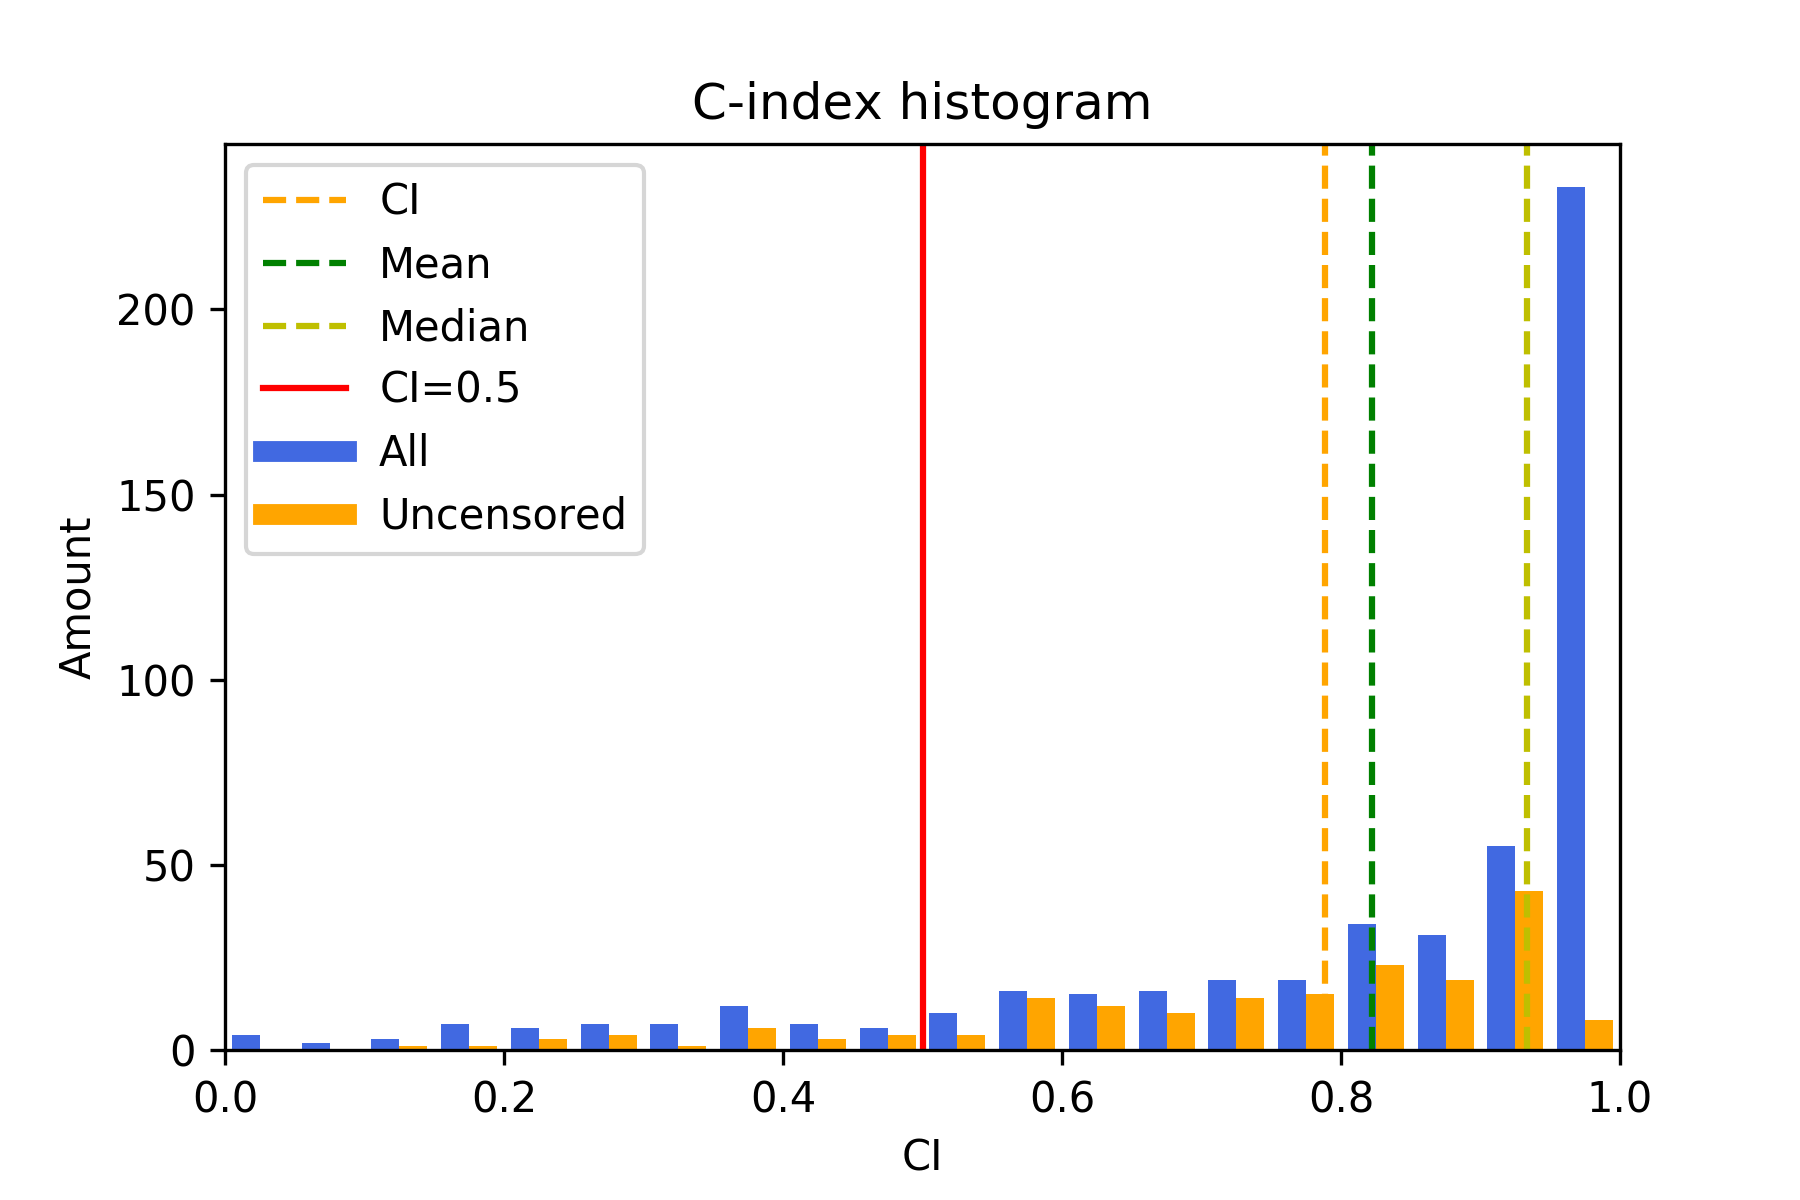
\includegraphics[width=.8\textwidth]{images/results/c-index_scalar}
  \caption[LOOCV scalar only model results]{
    Scalar only model results using \acrshort{LOOCV} \label{fig:results-scalar-LOOCV}
    
    Histogram showing the distribution of all the \acrshort{LOOCV} elements' \acrshort{CI}
    when using mixed pairs to obtain the \acrshort{CI}. 
    In blue the distribution of all the \acrshort{LOOCV} elements. In orange only the uncensored
    elements, which have more pairs to compare with.
  }
\end{figure}

\begin{figure}
  \centering
  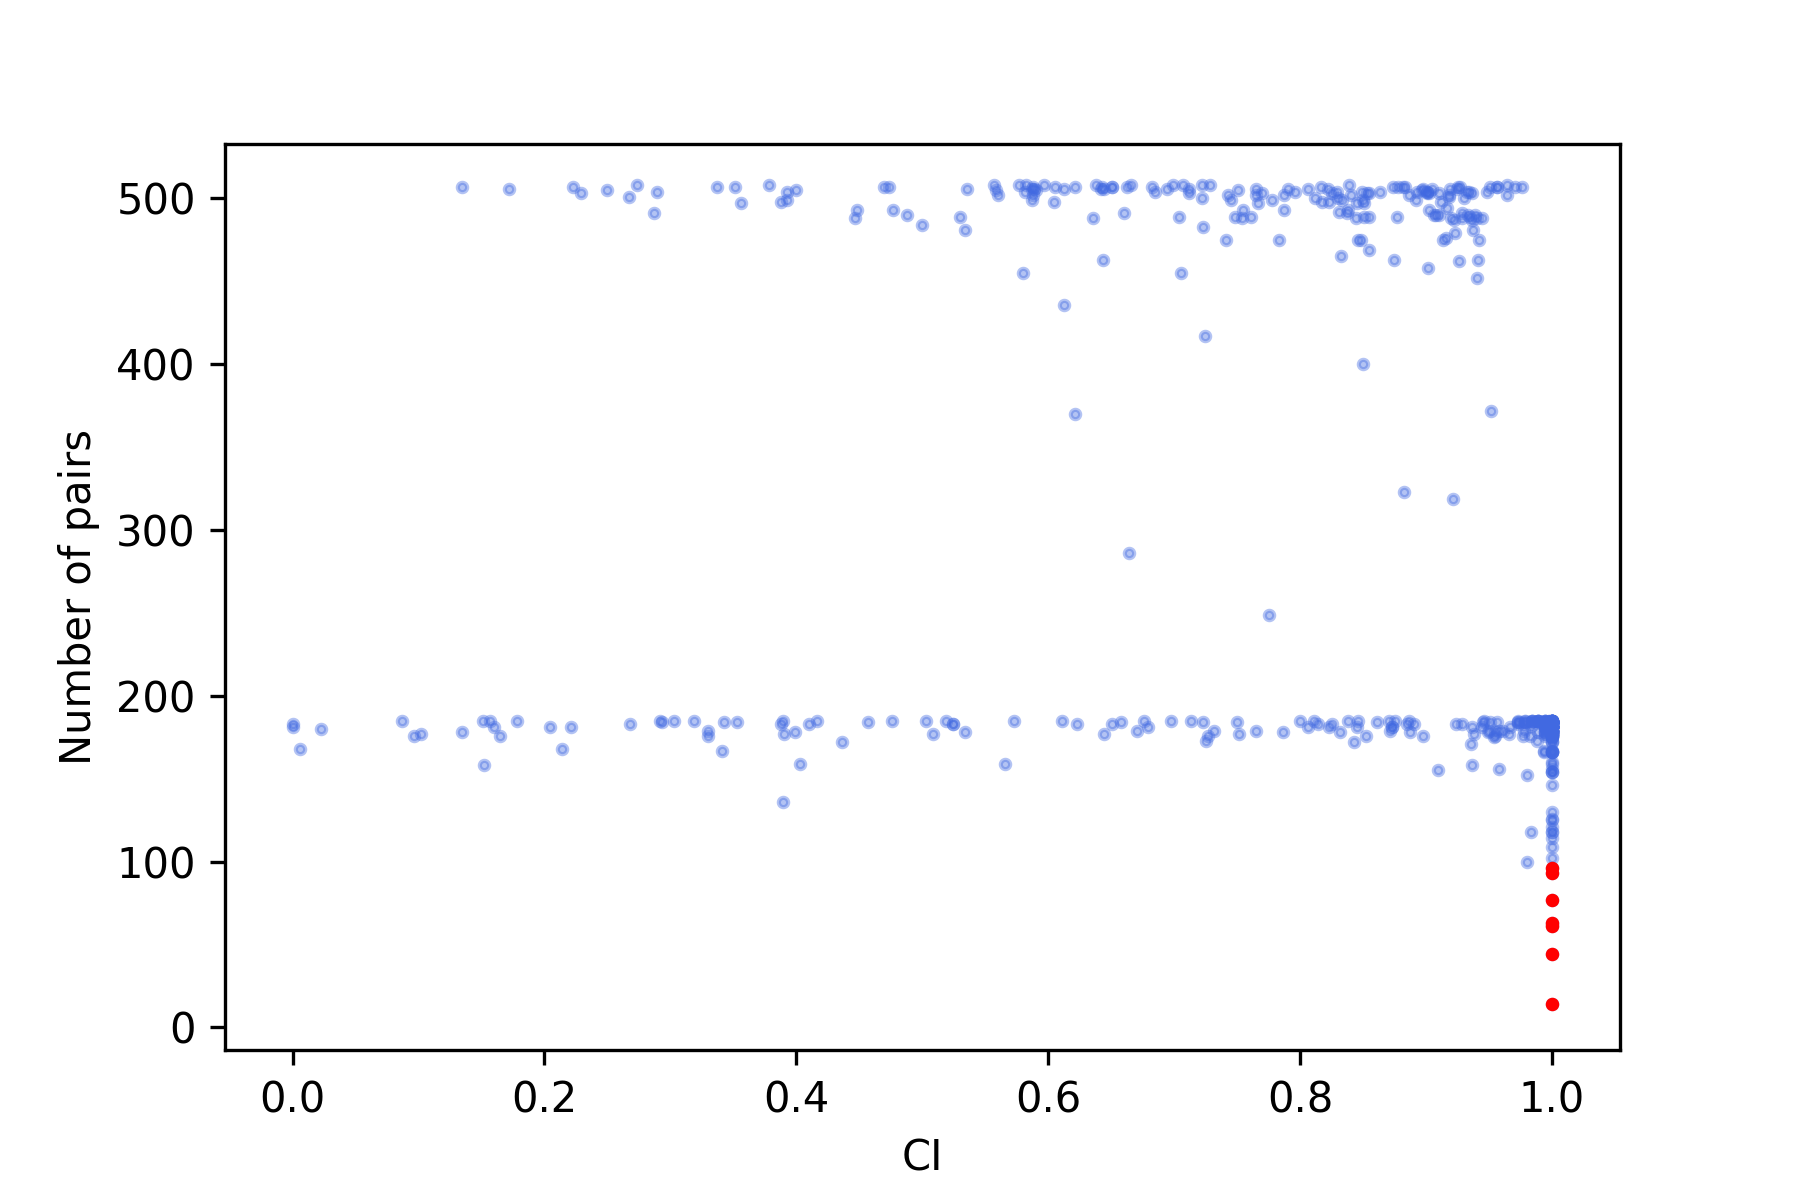
\includegraphics[width=.8\textwidth]{images/results/scatter_scalar}
  \caption[CI against pairs scatter plot]{
    Scatter plot of \acrshort{CI} against number of pairs for scalar only model
    \label{fig:scatter-scalar-CI}

    In red elements that have less than 100 pairs to compare with, and thus the \acrshort{CI} 
    can be close to 1.
  }
\end{figure}

\ssecc{Build deep siamese network}

This step is yet to be completed. Once the previous siamese models have been finished this
one can start as an improvement of the previous ones.

It can take at least one more week to complete this step.

\ssecc{Predict patients survival}

This step is yet to be completed. Once there is a working model that allows to compare two 
individuals to see which one lives more, the prediction of the survival time of the patients 
should be implemented.

This step should take at most one week to complete.

